%!TEX program = xelatex
%!TEX TS-program = xelatex
%!TEX encoding = UTF-8 Unicode

\documentclass[a4paper]{article}
\usepackage[UTF8, heading = false, scheme = plain]{ctex}
\usepackage{graphicx}
\usepackage{cite}
\usepackage{geometry}
\geometry{left=2.0cm, right=2.0cm, top=2.5cm, bottom=2.5cm}
\usepackage[colorlinks,linkcolor=red,anchorcolor=blue,citecolor=green]{hyperref}
\usepackage{subfig}
\usepackage{caption}
\captionsetup{font={scriptsize}}

\renewcommand\figurename{图}

%%%% 段落首行缩进两个字 %%%%
\makeatletter
\let\@afterindentfalse\@afterindenttrue
\@afterindenttrue
\makeatother
\setlength{\parindent}{2em}  %中文缩进两个汉字位

%%%% 下面的命令设置行间距与段落间距 %%%%
\linespread{1.4}
% \setlength{\parskip}{1ex}
\setlength{\parskip}{0.5\baselineskip}

\title{学习汇报\\第五周}
\author{熊凯亚}
\date{\today}

\begin{document}
\maketitle

\paragraph{回顾}
上周看了一些关于Collaborative Deep Learning的隐私问题,另一方面Google也提出了类似的概念,称为联合学习。在联合学习中,参与者在移动设备中存储所有的训练数据,在本地训练数据,然后将训练得到的更新(Updates)上传到云端,其他参与者下载更新到自己的移动设备,提高训练模型的准确性,利用这种方式联合学习解决了以前模型只能云端下发训练好的模型,而无法在本地训练的问题。联合学习的过程为:移动设备下载云端最新的共享模型,根据移动设备上用户的历史数据来改进和训练这个模型,然后将用户个性化的模型抽取为一个小的更新文件。仅将模型的差异部分上传到云端,同时使用加密算法保证其安全性,并在云端和其它用户上传的模型差异做平均化的更新,以改善共享模型。这样做的好处是,所有的训练数据都在用户的手机上,并不发送隐私信息到云端,仅仅发送的是模型的变更部分。联合学习过程如图所示。
\begin{figure*}[!ht]
\centering
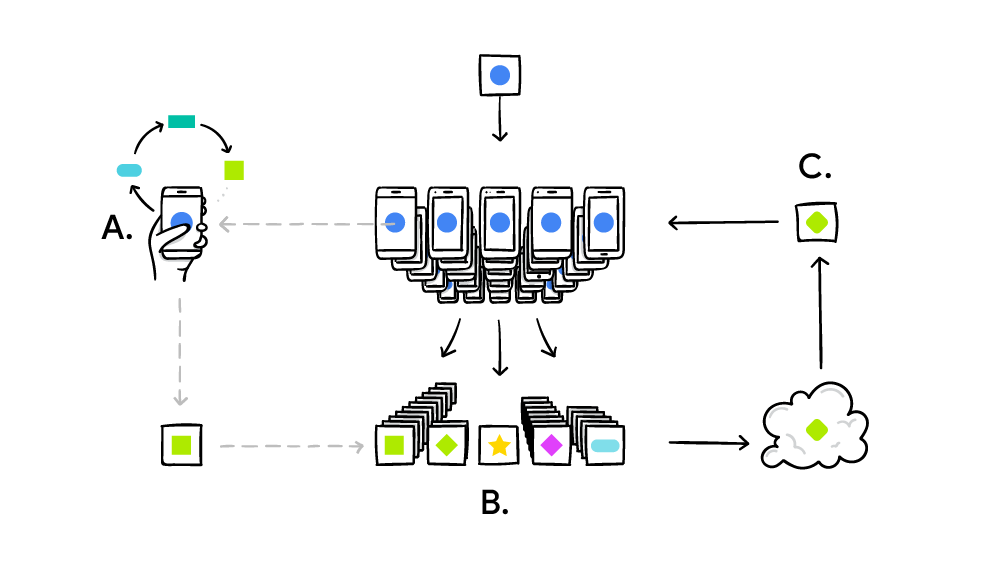
\includegraphics[width = \linewidth]{fig/FederatedLearningFlow}
\caption{联合学习流程图:A 根据手机的使用情况,对本地模型进行个性化设置并训练上传模型更新;B 许多用户的模型更新被聚集在一起;C 优化共享模型,然后很多用户又对新的模型进行下载、训练,并重复这个过程。}
\label{fig:Google}
\end{figure*}

\clearpage
\paragraph{联合学习的隐私问题}
对于联合学习的隐私问题,\cite{bonawitz2017practical}提出了一种能够保护用户隐私的安全聚集算法。不同于协作学习,联合学习中的参与者是一些移动设备,这些移动设备有一些特殊的属性,比如随意性,移动设备会随时失去网络连接,随时退出模型的训练等等。

联合学习原理安全聚集算法原理如下:中心化学习中,用户设备和云端模型交互,使用设备数据提高模型的准确性。联合学习中,用户设备下载云端模型,并在本地使用设备数据训练模型,并上传至云端更新模型。联合学习中,假设云服务提供商(Google)为恶意敌手。使用了安全聚集算法之后,模型更新的聚集由虚拟的第三方通过安全多方计算来完成,这就保证了云服务提供商对聚集的模型更新的不可知性。
\begin{figure*}[!h]
\begin{tabular}{ccc}
\subfloat[传统中心化云端训练模型]{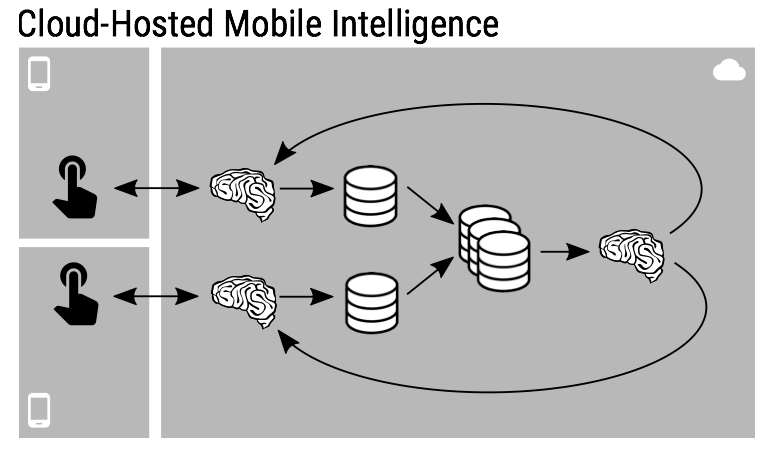
\includegraphics[width = 2in]{fig/Cloud-Hosted_Mobile_Intelligence.png}}&
\subfloat[联合学习]{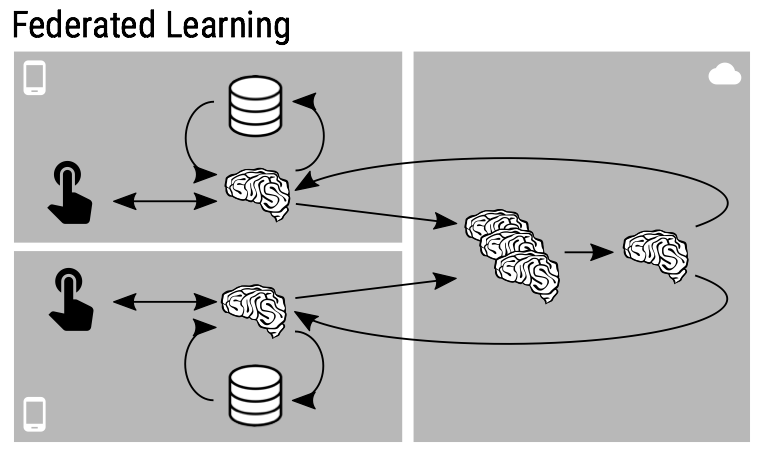
\includegraphics[width = 2in]{fig/Federated_Learning.png}}&
\subfloat[使用安全聚集的联合学习]{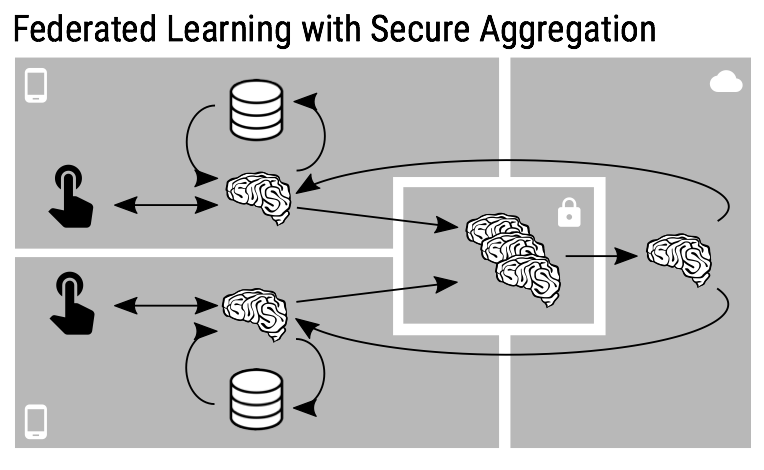
\includegraphics[width = 2in]{fig/Federated_Learning_with_Secure_Aggregation.png}}
\end{tabular}
\end{figure*}

安全聚集算法中,对于用户设备使用本地数据在本地训练的模型更新,使用秘密分享协议(Secret Sharing)将模型更新分为n份上传至云端服务器,并在服务器端使用安全多方计算,计算多个设备上传的模型更新。然后将计算结果添加到已有模型上,随后各个设备再继续下载最新的模型在本地训练,如此循环,直至模型收敛。

\paragraph{想法}
由于\cite{bonawitz2017practical}中只考虑了云服务提供商是恶意敌手,而没有考虑参与模型训练的设备有可能也是恶意敌手,所以可以在联合学习中参与者是否可以通过某种攻击方法攻击另外的参与者,进而获取模型的相关信息呢?

\bibliographystyle{IEEEtran}
\bibliography{references}
\end{document}


















